%===================================================================================
\chapter{Code Organization}\label{s:organization}
%===================================================================================

%----------------------------------
\section{SUNDIALS organization}\label{ss:sun_org}
%----------------------------------
% This is a shared SUNDIALS TEX file with description of
% the SUNDIALS organization
%
The family of solvers referred to as {\sundials} consists of the solvers
{\cvode} and {\arkode} (for ODE systems), {\kinsol} (for nonlinear algebraic
systems), and {\ida} (for differential-algebraic systems).  In addition,
{\sundials} also includes variants of {\cvode} and {\ida} with sensitivity analysis
capabilities (using either forward or adjoint methods), called {\cvodes} and
{\idas}, respectively.

The various solvers of this family share many subordinate modules.
For this reason, it is organized as a family, with a directory
structure that exploits that sharing (see Figures \ref{f:sunorg1} and
\ref{f:sunorg2}).
%%
%%
\begin{figure}[htb]
{\centerline{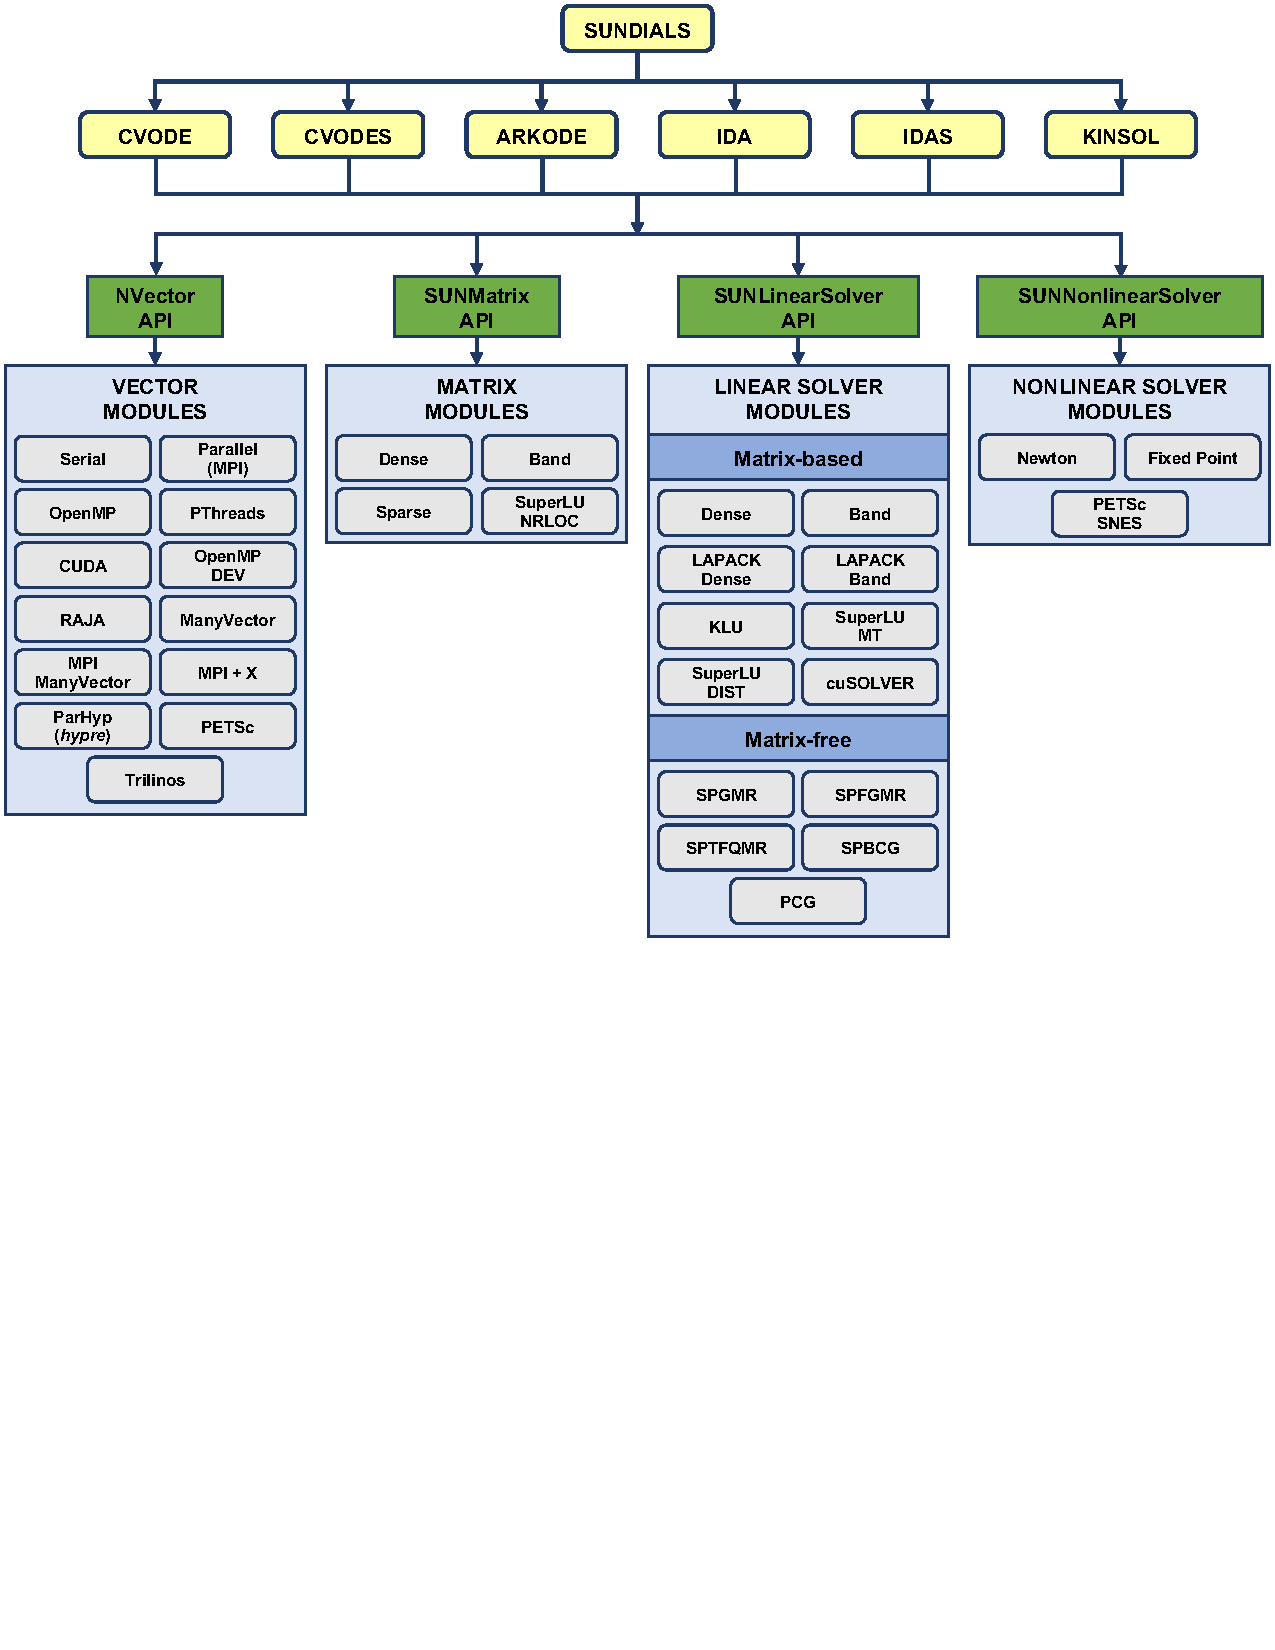
\includegraphics[width=\textwidth]{sunorg1}}}
\caption {High-level diagram of the {\sundials} suite.}\label{f:sunorg1}
\end{figure}
%%
%%
\begin{figure}[htb]
{\centerline{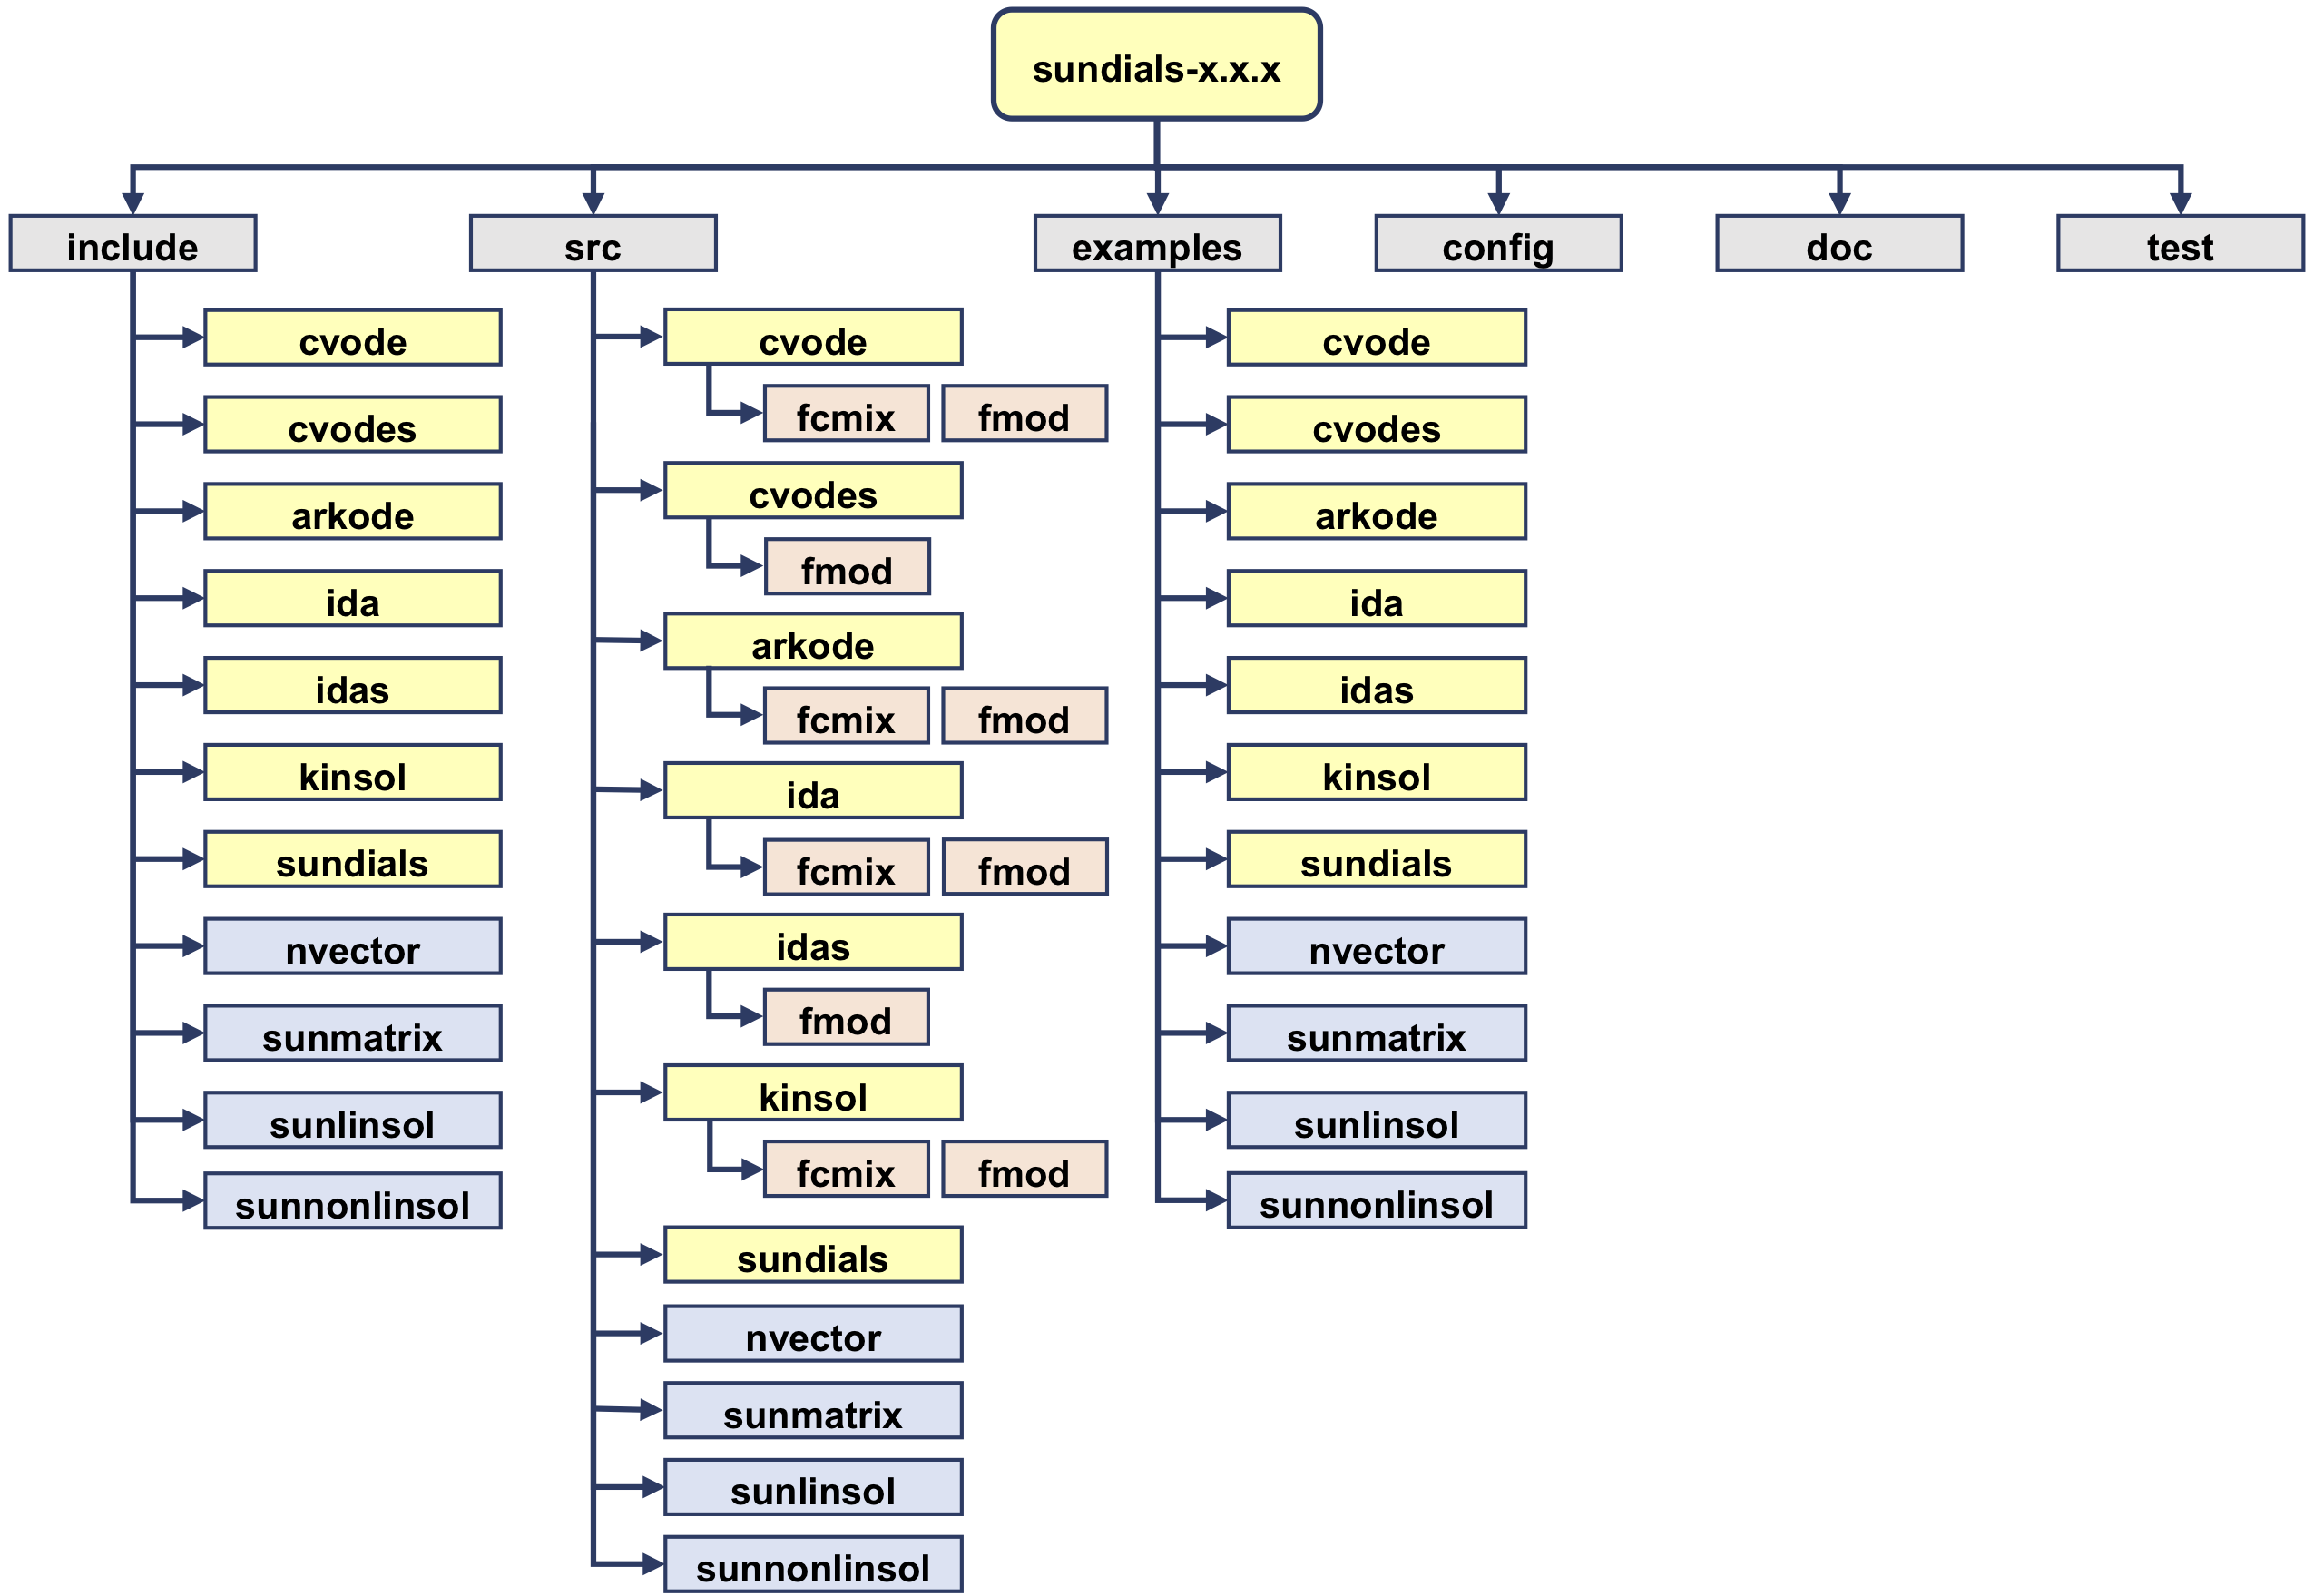
\includegraphics[width=\textwidth]{sunorg2}}}
\caption {Directory structure of the {\sundials} source tree.}\label{f:sunorg2}
\end{figure}
%%
%%
The following is a list of the solver packages presently available, and
the basic functionality of each:
\begin{itemize}

\item {\cvode},
  a solver for stiff and nonstiff ODE systems $dy/dt = f(t,y)$ based
  on Adams and BDF methods;

\item {\cvodes},
  a solver for stiff and nonstiff ODE systems with sensitivity analysis capabilities;

\item {\arkode},
  a solver for stiff, nonstiff, mixed stiff-nonstiff, and multirate ODE systems
  $M dy/dt = f_1(t,y) + f_2(t,y)$ based on Runge-Kutta methods;

\item {\ida},
  a solver for differential-algebraic systems $F(t,y,\dot{y}) = 0$ based on BDF methods;

\item {\idas},
  a solver for differential-algebraic systems
  with sensitivity analysis capabilities;

\item {\kinsol},
  a solver for nonlinear algebraic systems $F(u) = 0$.

\end{itemize}
Note for modules that provide interfaces to third-party libraries (i.e., LAPACK,
{\klu}, {\superlumt}, {\superludist}, {\hypre}, {\petsc}, {\trilinos}, and
{\raja}) users will need to download and compile those packages independently.


%----------------------------------
\section{KINSOL organization}\label{ss:kinsol_org}
%----------------------------------

\index{KINSOL@{\kinsol}!package structure}
The {\kinsol} package is written in the ANSI {\CC} language. This section
summarizes the basic structure of the package, although knowledge
of this structure is not necessary for its use.

The overall organization of the {\kinsol} package is shown in Figure
\ref{f:kinorg}.
\begin{figure}[!htb]
{\centerline{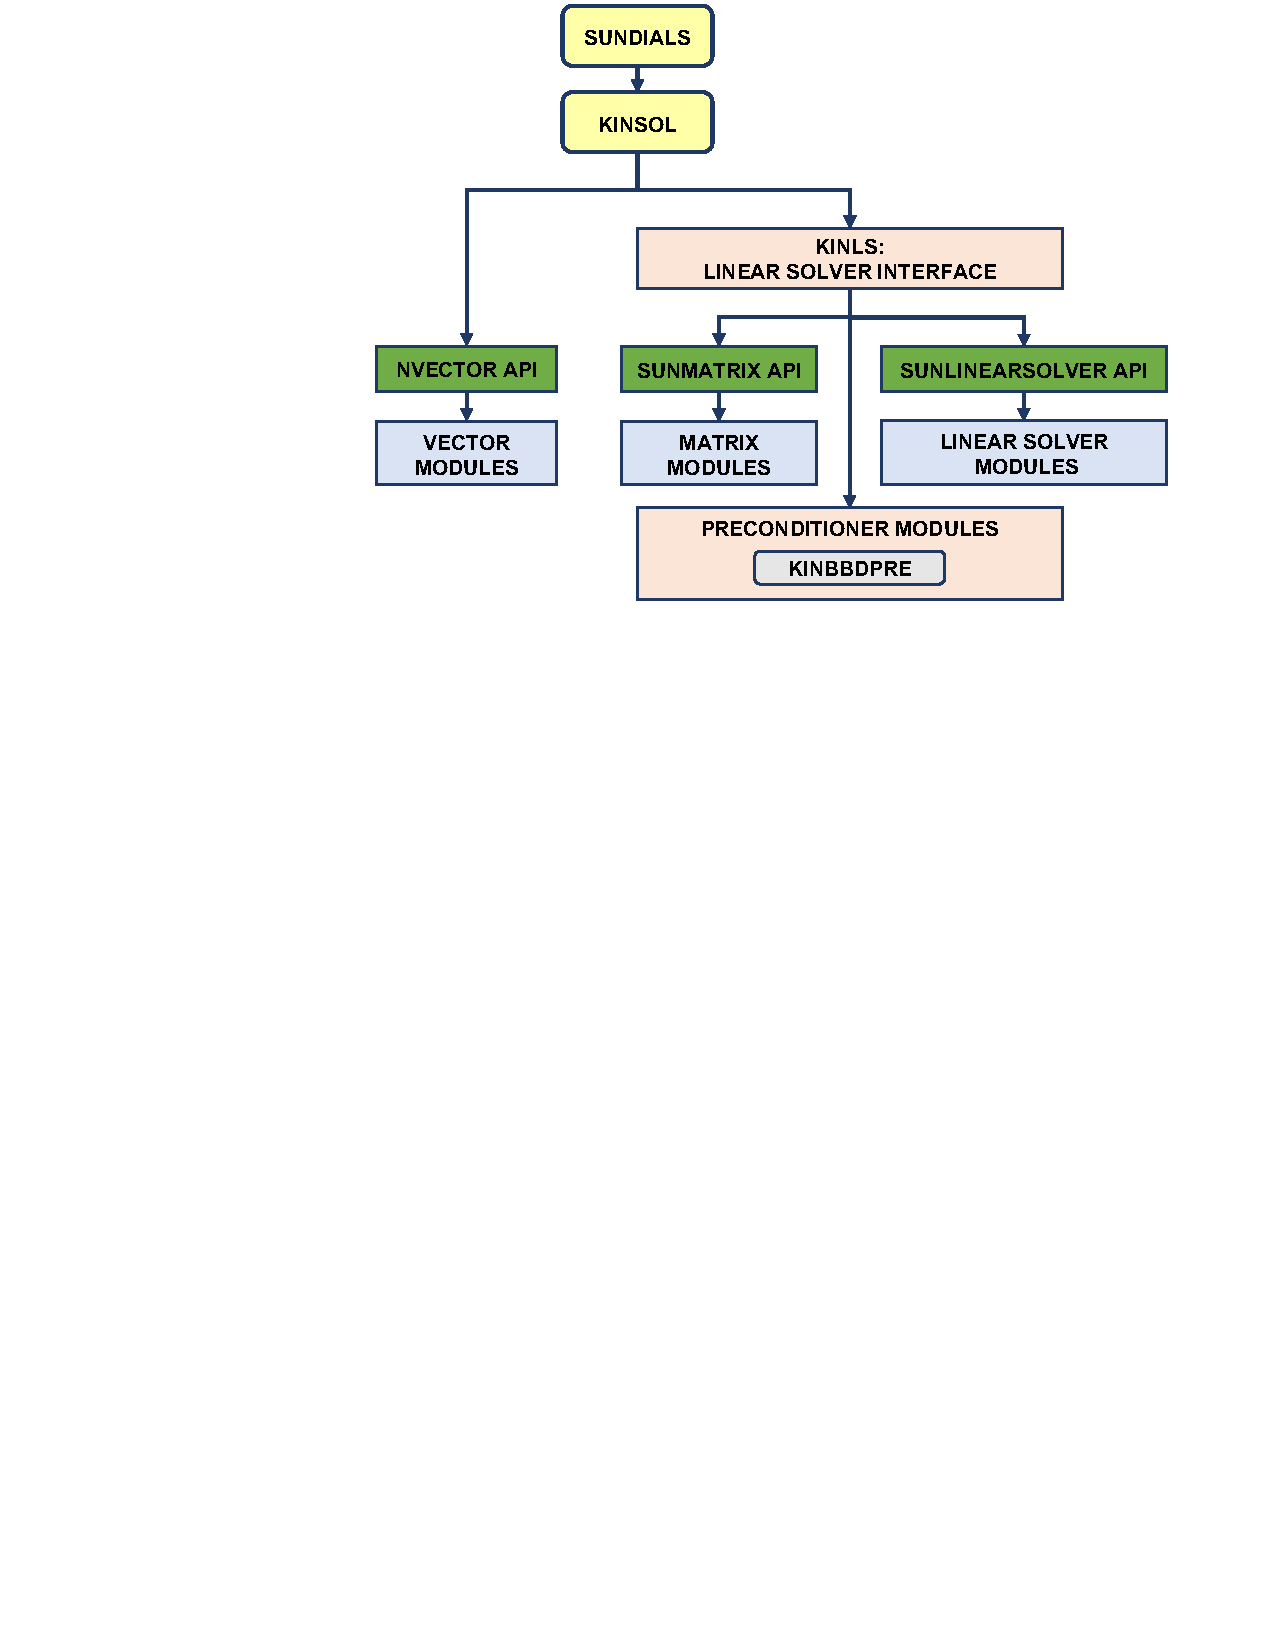
\includegraphics[width=\textwidth]{kinorg}}}
\caption [Overall structure diagram of the KINSOL package]
{Overall structure diagram of the {\kinsol} package.
  Modules specific to {\kinsol} begin with ``KIN'' ({\kinls} and {\kinbbdpre}),
  all other items correspond to generic {\sundials} vector, matrix, and solver
  modules (see Figure \ref{f:sunorg1}).}
\label{f:kinorg}
\end{figure}
The central solver module, implemented in the files
\id{kinsol.h}, \id{kinsol\_impl.h} and \id{kinsol.c}, deals with the solution
of a nonlinear algebraic system using either an Inexact Newton method or a
line search method for the global strategy. Although this module contains logic
for the Newton iteration, it has no knowledge of the method used to solve the
linear systems that arise. For any given user problem, one of the linear system
solver modules is specified, and is then invoked as needed.

\index{KINSOL@{\kinsol} linear solver interfaces|(}
{\kinsol} now has a single unified linear solver interface, {\kinls},
supporting both direct and iterative linear solvers built using the
generic {\sunlinsol} API (see Chapter \ref{s:sunlinsol}).  These
solvers may utilize a {\sunmatrix} object (see Chapter
\ref{s:sunmatrix}) for storing Jacobian information, or they may be
matrix-free. Since {\kinsol} can operate on any valid {\sunlinsol}
implementation, the set of linear solver modules available to
{\kinsol} will expand as new {\sunlinsol} modules are developed.

For users employing dense or banded Jacobian matrices, {\kinls}
includes algorithms for their approximation through difference
quotients, but the user also has the option of supplying the Jacobian
(or an approximation to it) directly.  This user-supplied
routine is required when using sparse or user-supplied Jacobian
matrices.

For users employing matrix-free iterative linear solvers, {\kinls}
includes an algorithm for the approximation by difference quotients of
the product between the Jacobian matrix and a vector, $Jv$. Again, the
user has the option of providing routines for this operation, in two
phases: setup (preprocessing of Jacobian data) and multiplication.

For preconditioned iterative methods, \index{preconditioning!setup and solve phases}
the preconditioning must be supplied by the user, again in two phases:
setup and solve.  While\index{preconditioning!advice on} there is no
default choice of preconditioner analogous to the difference-quotient
approximation in the direct case, the references
\cite{BrHi:89,Byr:92}, together with the example and demonstration
programs included with {\kinsol}, offer considerable assistance in
building preconditioners.

\index{KINSOL@{\kinsol} linear solvers!implementation details|(}
{\kinsol}'s linear solver interface consists of four primary phases,
devoted to (1) memory allocation and initialization, (2) setup of the
matrix data involved, (3) solution of the system, and (4) freeing of memory.
The setup and solution phases are separate because the evaluation of
Jacobians and preconditioners is done only periodically during the
solution, as required to achieve convergence. The call list within
the central {\kinsol} module to each of the associated functions is
fixed, thus allowing the central module to be completely independent
of the linear system method.
\index{KINSOL@{\kinsol} linear solvers!implementation details|)}

{\kinsol} also provides a preconditioner module called {\kinbbdpre} for use
with any of the Krylov iterative linear solvers. It works in conjunction
with {\nvecp} and generates a preconditioner that is
a block-diagonal matrix with each block being a banded matrix, as
further described in \S\ref{sss:kinbbdpre}.

All state information used by {\kinsol} to solve a given problem is saved
in a structure, and a pointer to that structure is returned to the
user.  There is no global data in the {\kinsol} package, and so, in this
respect, it is reentrant. State information specific to the linear
solver is saved in a separate structure, a pointer to which resides in
the {\kinsol} memory structure. The reentrancy of {\kinsol} was motivated
by the anticipated multicomputer extension, but is also essential
in a uniprocessor setting where two or more problems are solved by
intermixed calls to the package from within a single user program.
